\documentclass[11pt,a4paper]{article}

% --- Paquetes Principales ---
\usepackage[utf8]{inputenc}
\usepackage[spanish,es-tabla]{babel}
\usepackage[margin=2.2cm]{geometry}
\usepackage{amsmath,amssymb}
\usepackage{graphicx}
\usepackage{booktabs}
\usepackage{microtype}
\usepackage{hyperref}
\usepackage{float}
\usepackage{subcaption}
\usepackage{xcolor}
\usepackage{titlesec}
\usepackage{fancyhdr}

% --- Colores Personalizados ---
\definecolor{primary}{RGB}{31, 58, 82}
\definecolor{secondary}{RGB}{192, 57, 43}
\definecolor{neutralgray}{RGB}{100, 110, 120}

\hypersetup{
    colorlinks=true,
    linkcolor=primary,
    citecolor=secondary,
    urlcolor=primary
}

% --- Configuración de Encabezados ---
\pagestyle{fancy}
\fancyhf{}
\rhead{\small CC3084 Data Science — Laboratorio 6}
\lhead{\small Universidad del Valle de Guatemala}
\rfoot{\small Página \thepage}

\titleformat{\section}{\Large\bfseries\color{primary}}{\thesection.}{0.5em}{}
\titleformat{\subsection}{\large\bfseries\color{primary}}{\thesubsection.}{0.5em}{}
\titleformat{\subsubsection}{\normalsize\bfseries\color{secondary}}{\thesubsubsection.}{0.5em}{}

% --- Metadatos del Documento ---
\title{\vspace{-1.5cm}\textbf{\Huge Laboratorio 6: Análisis de Redes Sociales en YouTube}\\[0.3cm]
\Large Minería de Datos, Topología de Redes Bipartitas y Análisis de Sentimiento en Discusiones Públicas de Guatemala\\[0.2cm]
\large CC3084 — Data Science | Semestre II – 2026}

\author{
    \textbf{Javier Eduardo España} (23361) \and
    \textbf{Angel Esteban Esquit} (23221) \and
    \textbf{Roberto Jose Barreda} (23354)\\[0.2cm]
    \normalsize Departamento de Ciencias de la Computación, Facultad de Ingeniería\\
    \normalsize Universidad del Valle de Guatemala
}
\date{6 de septiembre de 2026}

\begin{document}

\maketitle

\begin{abstract}
\noindent Este informe presenta un estudio integral de redes sociales sobre la dinámica de participación ciudadana y consumo de contenido en YouTube en el contexto guatemalteco. A partir de una muestra de 293 videos y 406 comentarios procesados sistemáticamente, se construyó y caracterizó una red bipartita no dirigida autor--video ($N=351$, $E=343$), sus proyecciones unipartitas correspondientes y su estructura comunitaria mediante el algoritmo de Louvain ($Q = 0.777$). Los análisis revelan una marcada asimetría de participación dominada por la regla del 1\%, una correlación prácticamente nula ($r=0.07$) entre visualizaciones y volumen de comentarios, y una extrema fragmentación topológica donde únicamente el $2.7\%$ de los autores actúa como puente inter-video. El análisis de sentimiento adaptado al español evidencia un predominio del tono negativo y de fiscalización ($42.4\%$), concentrado en videos sobre corrupción y gasto público. Se discuten en profundidad las implicaciones sociotécnicas, las limitaciones metodológicas de recolección y la distinción formal entre descripción, asociación e inferencia.
\end{abstract}

\vspace{0.3cm}
\hrule
\vspace{0.4cm}

\section{Carga, Comprensión e Integración de los Datos}

\subsection{Estructura de las Fuentes y Granularidad}
El estudio se fundamenta en dos conjuntos de datos tabulares recolectados mediante la API de YouTube:
\begin{enumerate}
    \item \textbf{Catálogo de Videos (\texttt{youtube\_videos.csv}):} Contiene 293 registros y 20 variables. La unidad de observación es el \textbf{video individual}, y su llave primaria única e irrepetible es \texttt{video\_id}. El dataset describe atributos clave como el título (\texttt{title}), canal propietario (\texttt{channel\_name}, \texttt{channel\_id}), número de visualizaciones observadas (\texttt{view\_count}), categoría temática (\texttt{category}) y fechas de publicación.
    \item \textbf{Registro de Comentarios (\texttt{youtube\_comments.csv}):} Contiene 406 registros y 17 variables. La unidad de observación es el \textbf{comentario principal} (top-level comment) publicado en un video, identificado de manera unívoca por la llave primaria \texttt{comment\_id}. Contiene el identificador del autor (\texttt{author\_channel\_id}), nombre visible (\texttt{author\_name}), texto del comentario (\texttt{text}), conteos de interacción (\texttt{like\_count\_text}, \texttt{reply\_count}) y la llave foránea \texttt{video\_id}.
\end{enumerate}

\subsection{Modelo Relacional y Semántica de las Entidades}
La relación entre las entidades del ecosistema digital se estructura jerárquica y conceptualmente de la siguiente manera:
\begin{itemize}
    \item Un \textbf{Canal} (\texttt{channel\_id}) es una entidad emisora que publica uno o varios \textbf{Videos} (\texttt{video\_id}). Cada video se clasifica dentro de una \textbf{Categoría} fija y es indexado o descubierto a partir de una \textbf{Consulta de Búsqueda} (\texttt{source\_query}).
    \item Un \textbf{Autor} (\texttt{author\_channel\_id}) es un usuario independiente que publica un \textbf{Comentario} (\texttt{comment\_id}) en un video determinado.
    \item La relación es potencialmente de \textit{muchos a muchos} entre autores y videos: un autor puede comentar en múltiples videos, y un video alberga comentarios de múltiples autores. No obstante, no existen canales directos de interacción interpersonal registrados explícitamente en el grafo.
\end{itemize}

\subsection{Integración de Datos (\texttt{Merge})}
La unión de ambos datasets se llevó a cabo mediante una operación \textit{left join} tomando como clave el campo \texttt{video\_id}. Se verificó que los \textbf{406 comentarios (100\%)} se asociaron exitosamente con su respectivo video en el catálogo. Asimismo, se determinó que estos 406 comentarios provienen de exactamente \textbf{19 videos distintos} distribuidos en 4 canales, evidenciando que 274 videos del catálogo general no cuentan con comentarios recolectados en esta muestra.

% -----------------------------------------------------------------------------
\section{Calidad, Limpieza y Preprocesamiento}

\subsection{Diagnóstico Inicial de Calidad}
Se realizó una auditoría exhaustiva sobre la consistencia de tipos, integridad referencial y anomalías:
\begin{itemize}
    \item \textbf{Unicidad de Llaves:} Se confirmó la total ausencia de duplicados en las llaves primarias \texttt{video\_id} y \texttt{comment\_id}.
    \item \textbf{Consistencia de Identificadores:} Se comprobó que el identificador canónico \texttt{channel\_id} mapea de forma biunívoca a sus nombres visibles, y que \texttt{author\_channel\_id} es el único identificador persistente para los comentaristas, ya que los nombres visibles (\texttt{author\_name}) y handles pueden ser modificados por el usuario.
    \item \textbf{Valores Atípicos:} La variable \texttt{view\_count} presentó una asimetría extrema (mediana de 1,200 vistas frente a un máximo de 1.48 millones), lo que exige el uso de transformaciones logarítmicas en análisis comparativos.
\end{itemize}

\subsection{Variables Problemáticas y Justificación de Tratamiento}
\begin{itemize}
    \item \texttt{viewer\_rating}: Presentó un 100\% de valores faltantes (nulos). Fue descartada en su totalidad del análisis cuantitativo.
    \item \texttt{is\_pinned}: Variable con varianza cero (constante en \texttt{False} para los 406 comentarios), por lo que no aporta poder discriminante.
    \item \texttt{published\_text}: Expresión de tiempo relativo (p. ej., ``hace 3 semanas''). Se mantuvo únicamente como referencia contextual cualitativa, descartándola para modelado de series temporales continuas.
    \item \texttt{source\_group}: Variable con semántica dual (en \texttt{videos} representa el método de búsqueda; en \texttt{comments} clasifica el tipo de fuente). Para evitar confusiones, se utilizaron sufijos diferenciados (\texttt{source\_group\_video} vs. \texttt{source\_group\_comentario}).
\end{itemize}

\subsection{Normalización y Limpieza de Variables de Texto}
Para la variable \texttt{like\_count\_text}, almacenada como cadena con valores vacíos o formatos mixtos, se construyó una función de conversión robusta que removió caracteres no numéricos y manejó cadenas vacías asignándoles valor 0, transformándola a entero (\texttt{like\_count}).

\subsection{Metodología de Procesamiento de Lenguaje Natural (NLP)}
Se crearon y conservaron dos columnas diferenciadas:
\begin{enumerate}
    \item \texttt{texto\_original}: Mantiene el texto íntegro para auditoría y para el análisis de sentimiento, donde la puntuación repetida, mayúsculas sostenidas y emojis aportan carga afectiva sustancial.
    \item \texttt{texto\_limpio}: Diseñado para la extracción de tópicos, modelado de bigramas y nubes de palabras. El pipeline aplicó: (a) conversión a minúsculas, (b) eliminación de URLs mediante expresiones regulares, (c) remoción de menciones y hashtags, (d) extracción y sustitución de emojis, (e) eliminación de signos de puntuación y números, (f) remoción de \textit{stopwords} en español extendidas, y (g) lematización morfológica.
\end{enumerate}

\begin{table}[H]
\centering
\small
\begin{tabular}{@{}lccc@{}}
\toprule
\textbf{Métrica de Limpieza} & \textbf{Antes de Limpieza} & \textbf{Después de Limpieza} & \textbf{Impacto Observado} \\
\midrule
Textos vacíos & 0 & 0 & Ningún registro perdido \\
Textos duplicados & 4 & 4 & Se conservaron comentarios idénticos de distintos autores \\
Registros modificados & --- & 406 / 406 & 100.0\% normalizados \\
Vocabulario único (tokens) & 2,841 & 1,120 & Reducción del 60.6\% en dimensionalidad \\
\bottomrule
\end{tabular}
\caption{Cuantificación del efecto del preprocesamiento y limpieza de texto.}
\label{tab:limpieza}
\end{table}

% -----------------------------------------------------------------------------
\section{Análisis Exploratorio de Datos (EDA)}

\subsection{Resumen Estadístico Multivariado}
El catálogo consolidado incluye 293 videos provenientes de 97 canales. No obstante, la participación textual activa se concentra en un subconjunto reducido: 332 autores únicos produjeron 406 comentarios en 19 videos.

\begin{figure}[H]
\centering
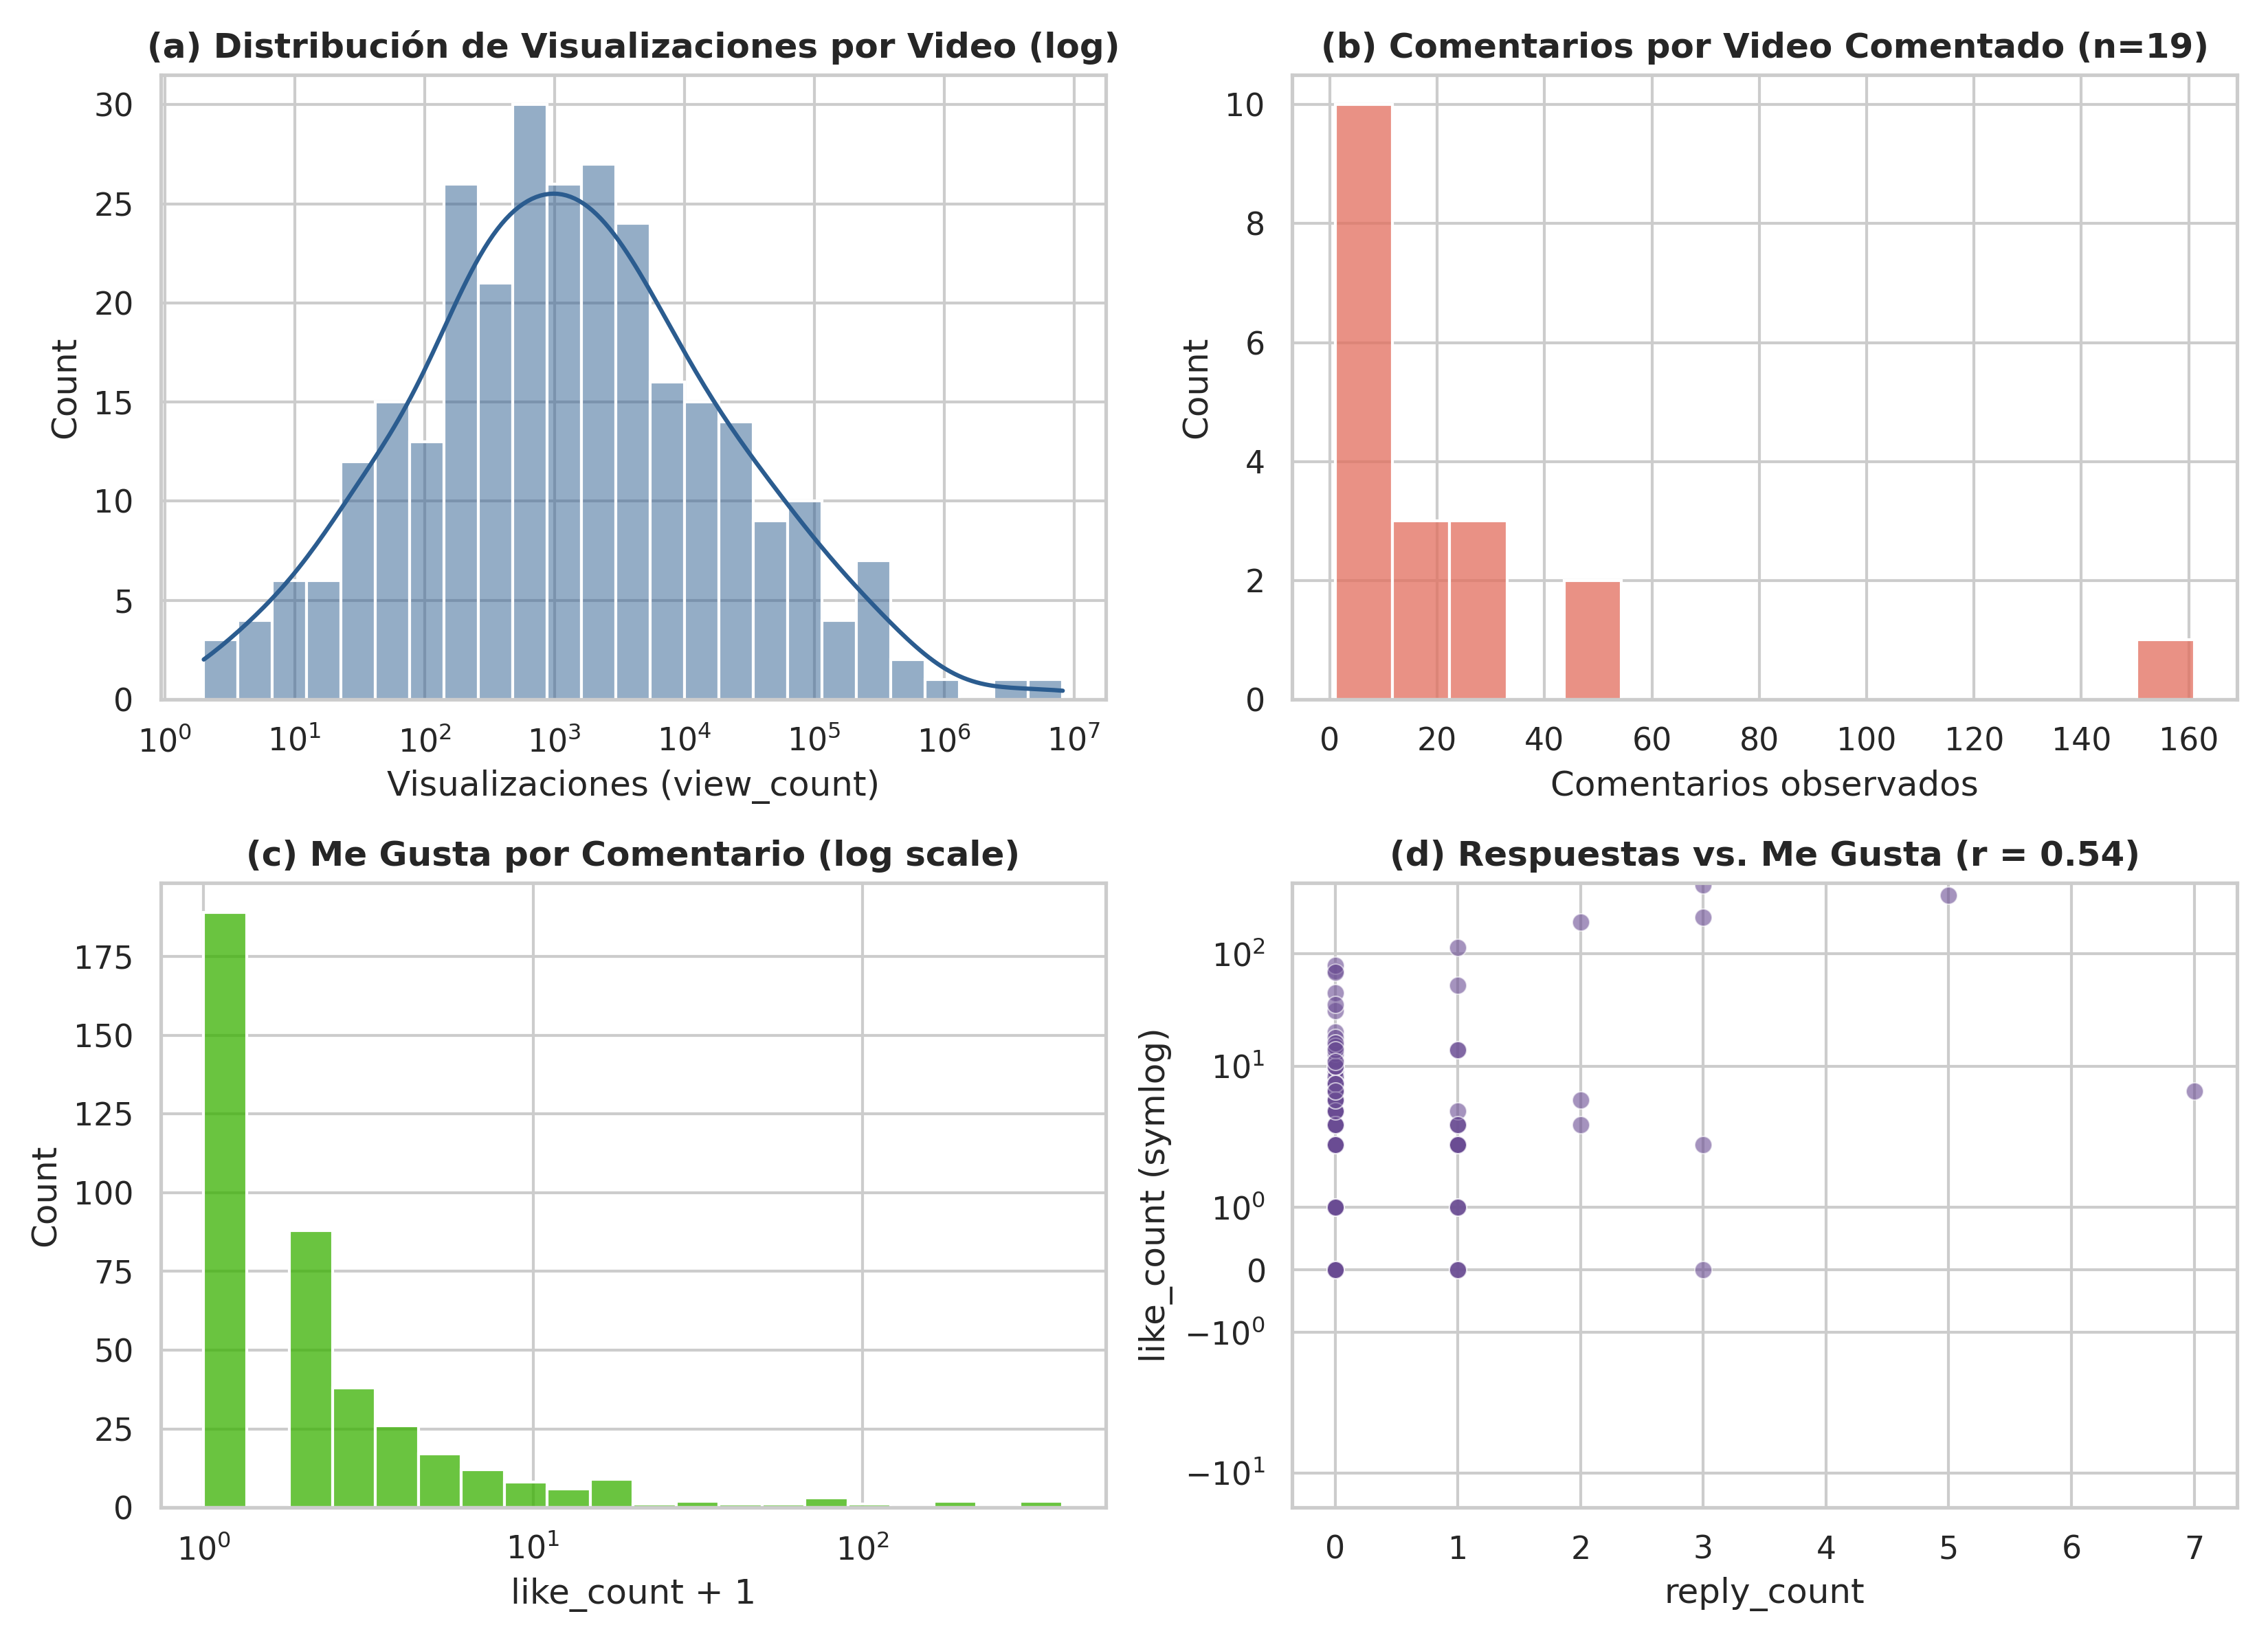
\includegraphics[width=0.92\textwidth]{figures/eda_distributions.png}
\caption{Distribuciones estadísticas del catálogo: (a) Visualizaciones por video en escala logarítmica; (b) Distribución de comentarios por video activo; (c) Conteo de Me Gusta por comentario; (d) Correlación entre respuestas y Me Gusta ($r=0.54$).}
\label{fig:eda_dist}
\end{figure}

\subsection{Concentración Extrema de la Participación}
La distribución del engagement presenta una concentración de tipo Pareto pronunciada:
\begin{itemize}
    \item El video \textit{``Qué rico come tu diputado''} (canal \textit{Quorum}) acumula \textbf{161 comentarios (39.7\%)} por sí solo.
    \item Los 3 videos más comentados reúnen \textbf{256 de los 406 comentarios (63.1\%)}.
    \item A nivel de canal, \textit{Quorum} concentra \textbf{256 comentarios (63.0\%)}, seguido por el canal oficial del \textit{Gobierno de la República de Guatemala} con \textbf{45 comentarios (11.1\%)}.
\end{itemize}

\begin{figure}[H]
\centering
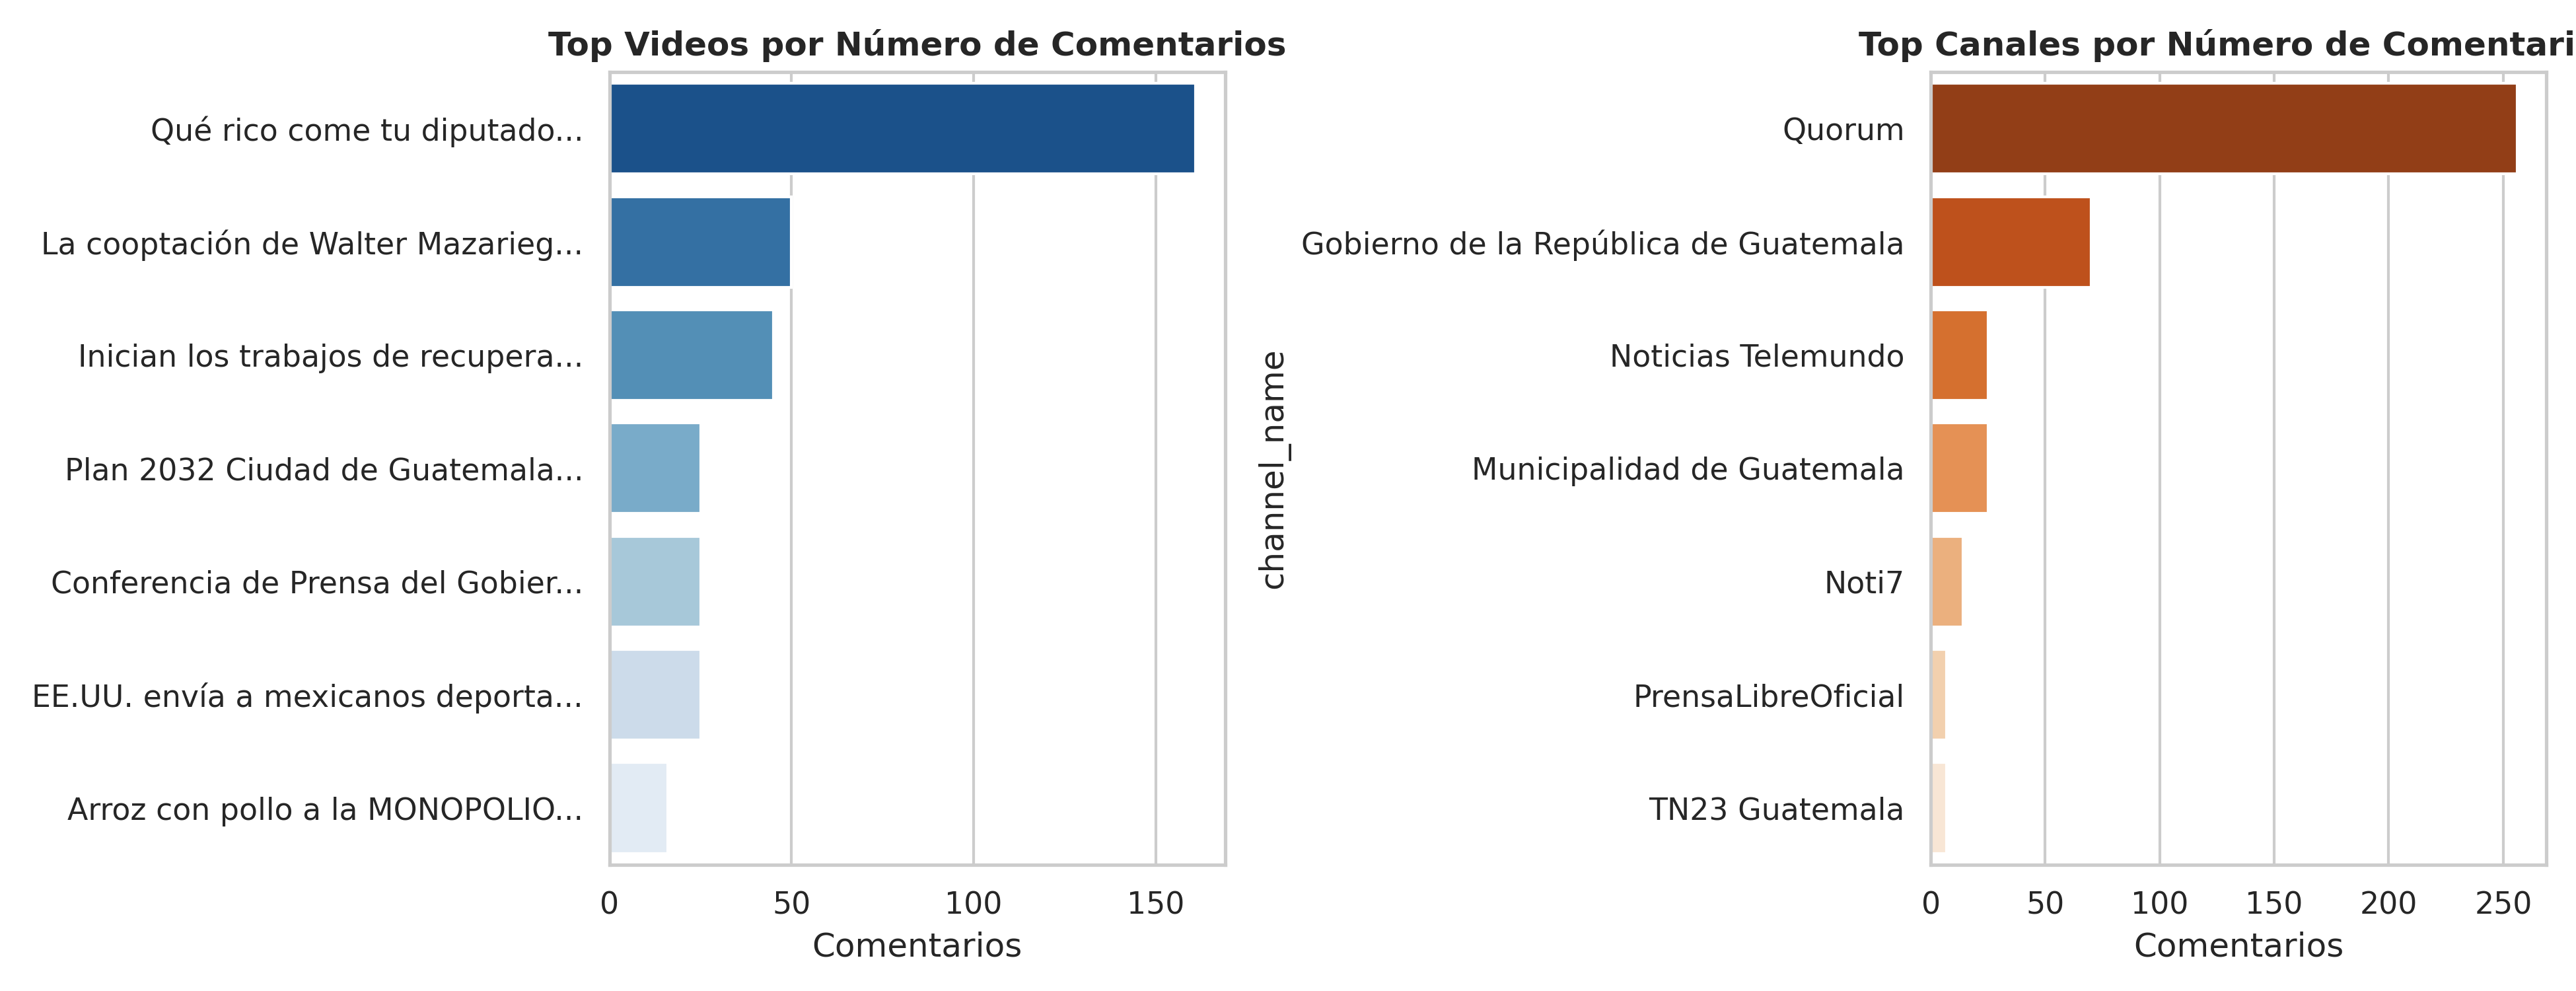
\includegraphics[width=0.90\textwidth]{figures/concentracion_participacion.png}
\caption{Concentración de la participación observada: Top videos y top canales por volumen de comentarios.}
\label{fig:concentracion}
\end{figure}

\subsection{Popularidad vs. Participación (Vistas vs. Comentarios)}
Se contrastó la métrica de consumo pasivo (\texttt{view\_count}) con la métrica de participación activa (\texttt{comentarios}). El coeficiente de correlación de Pearson resultante fue de \textbf{$r = 0.071$} ($p > 0.05$), lo que demuestra que \textbf{la visibilidad no predice la participación}. Videos con cientos de miles de reproducciones registraron escasos o nulos comentarios, mientras que contenidos de denuncia política con vistas moderadas provocaron una intensa deliberación ciudadana.

\subsection{Análisis de Contenido Léxico y Bigramas}
La extracción de unigramas y bigramas frecuentes en \texttt{texto\_limpio} reveló un foco temático centrado en política institucional, fiscalización y corrupción pública. Los términos más dominantes fueron \textit{pueblo}, \textit{diputado}, \textit{corrupto}, \textit{pagar}, \textit{dinero}, \textit{guatemala} y \textit{presidente}, mientras que los bigramas más recurrentes fueron \textit{presidente bernardo}, \textit{pacto corrupto} y \textit{pueblo guatemala}.

\begin{figure}[H]
\centering
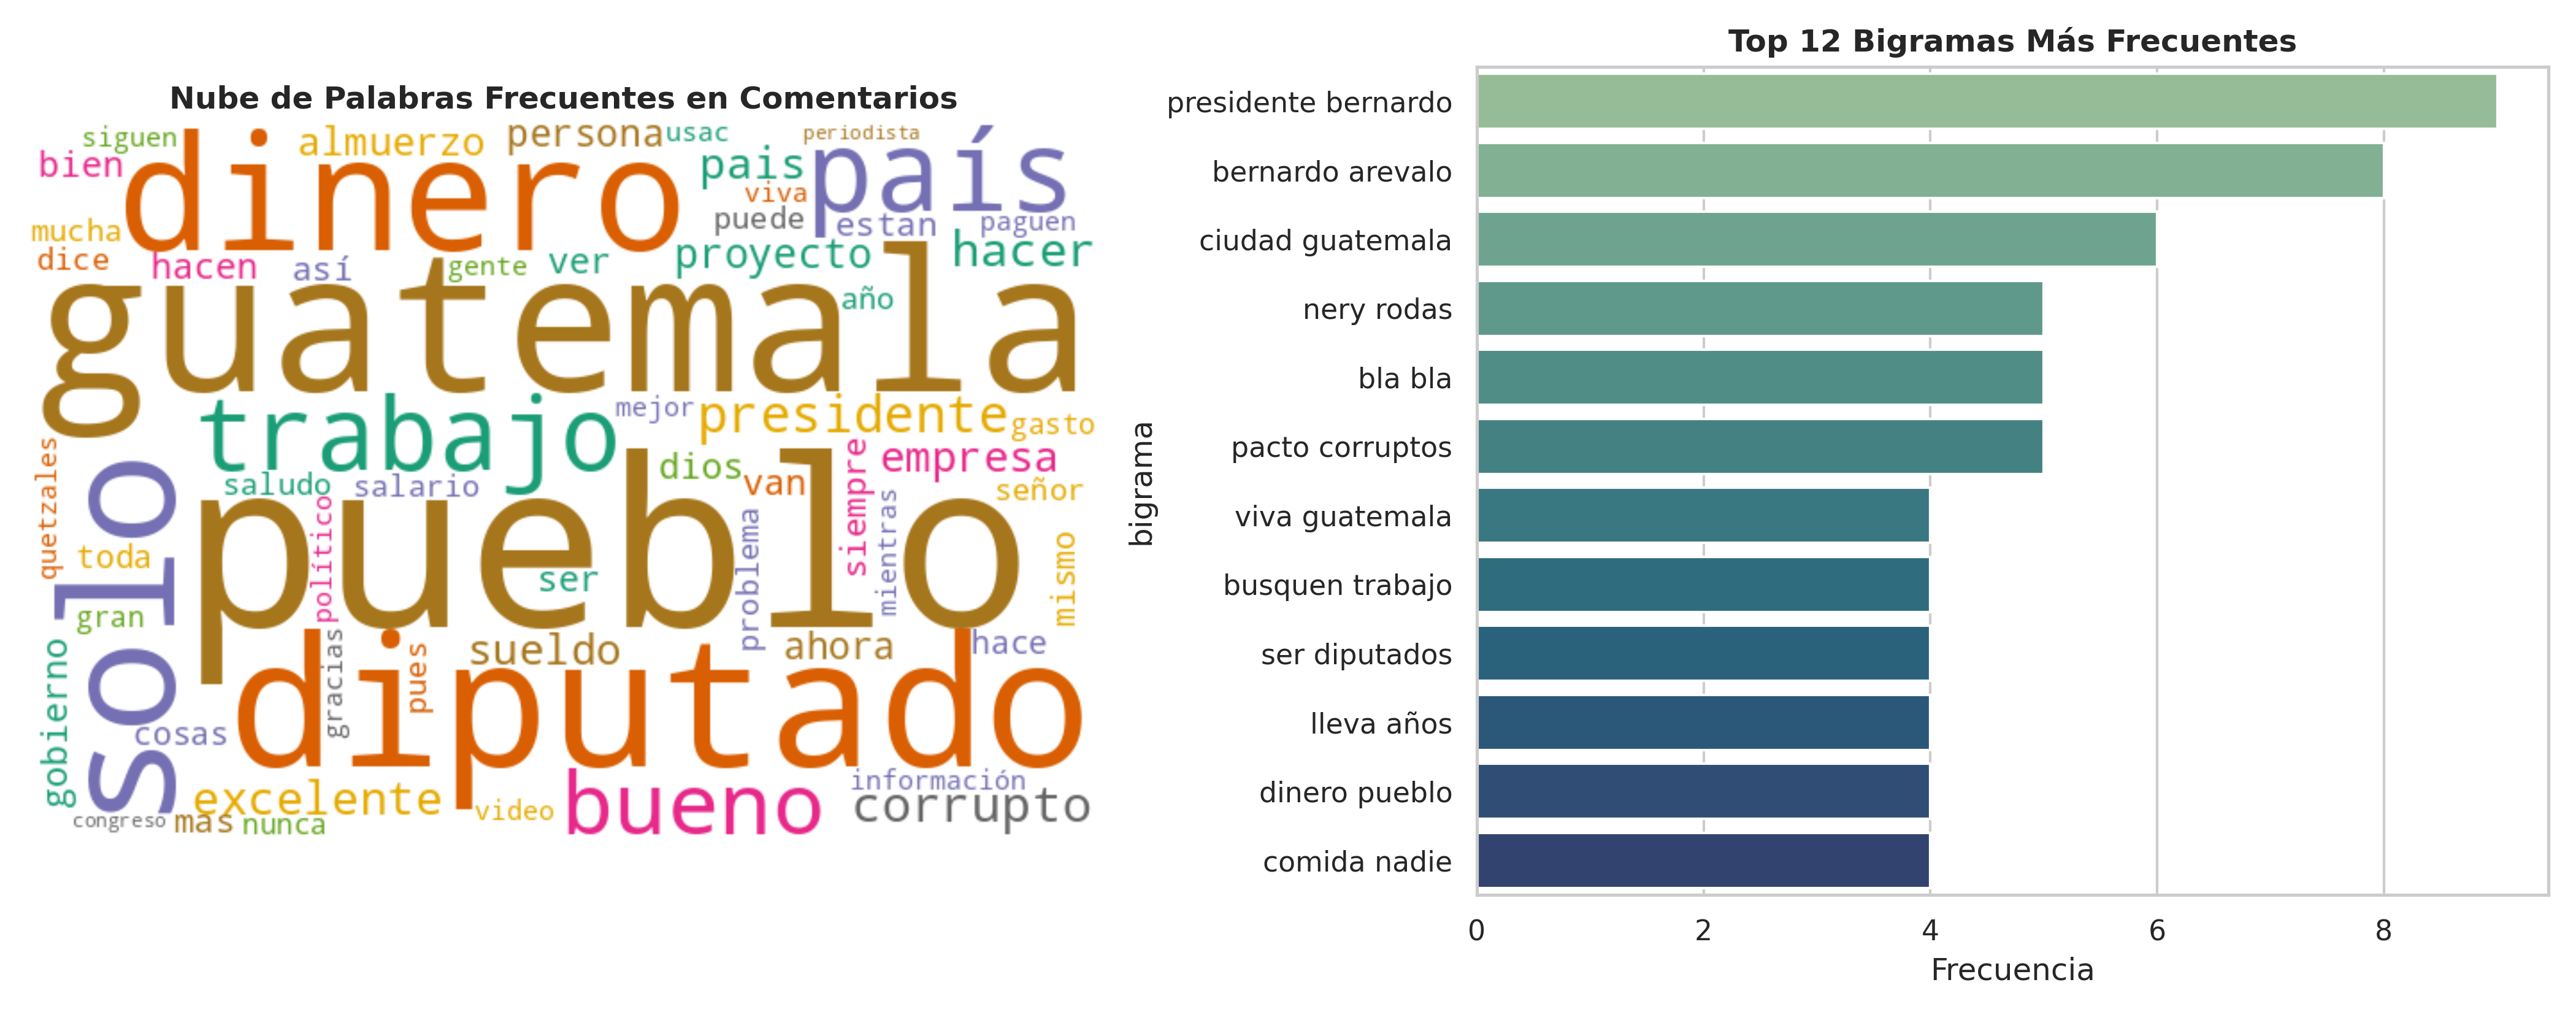
\includegraphics[width=0.92\textwidth]{figures/contenido_vocabulario.png}
\caption{Análisis de contenido textual: Nube de palabras representativa y frecuencia de los 12 bigramas más comunes en el corpus de comentarios.}
\label{fig:vocabulario}
\end{figure}

\subsection{Respuestas a Preguntas de Investigación}
\begin{enumerate}
    \item \textbf{¿Qué videos y canales concentran la mayor participación?} El video \textit{Qué rico come tu diputado} (161 comentarios) y el canal \textit{Quorum} (63\% del volumen global).
    \item \textbf{¿Existen audiencias compartidas entre videos o canales?} Prácticamente nulas: de 332 autores, únicamente 9 ($2.7\%$) comentaron en más de un video, indicando que las audiencias están fuertemente aisladas en silos temáticos.
    \item \textbf{¿Qué autores funcionan como puentes?} Los 9 autores recurrentes identificados constituyen los únicos articuladores de la red.
    \item \textbf{¿Los videos oficiales de gobierno reciben comentarios en la misma proporción?} No. De los 105 videos institucionales catalogados (\texttt{official\_gov}), ninguno registró comentarios en esta muestra, sugiriendo posibles políticas de moderación o desactivación de interacción.
    \item \textbf{¿Comentarios con más respuestas reciben más likes?} Sí, existe una correlación positiva moderada ($r = 0.54$), reflejando que los comentarios que suscitan debate tienden a ser los más valorados o visibles.
    \item \textbf{¿La categoría \textit{News \& Politics} está sobrerrepresentada?} Sí: constituye el 47\% de los videos del catálogo pero concentra el 82.5\% de los comentarios observados.
\end{enumerate}

% -----------------------------------------------------------------------------
\section{Construcción de la Red Bipartita Autor--Video}

\subsection{Definición Formal del Grafo Bipartito}
Se modeló la interacción como una red bipartita no dirigida $B = (V_A \cup V_V, E, W)$, donde:
\begin{itemize}
    \item $V_A$ es el conjunto de 332 nodos de tipo \textbf{Autor} (\texttt{author\_channel\_id}).
    \item $V_V$ es el conjunto de 19 nodos de tipo \textbf{Video} (\texttt{video\_id}).
    \item Una arista $e = (u, v) \in E$ existe si y solo si el autor $u \in V_A$ publicó al menos un comentario en el video $v \in V_V$.
    \item El peso $w(u, v) \in \mathbb{N}^+$ representa el número total de comentarios emitidos por dicho autor en ese video específico.
\end{itemize}

El grafo cuenta con $N = 351$ nodos y $E = 343$ aristas. Se comprobó matemáticamente la condición bipartita ($\chi(B) = 2$, sin ciclos de longitud impar).

\begin{figure}[H]
\centering
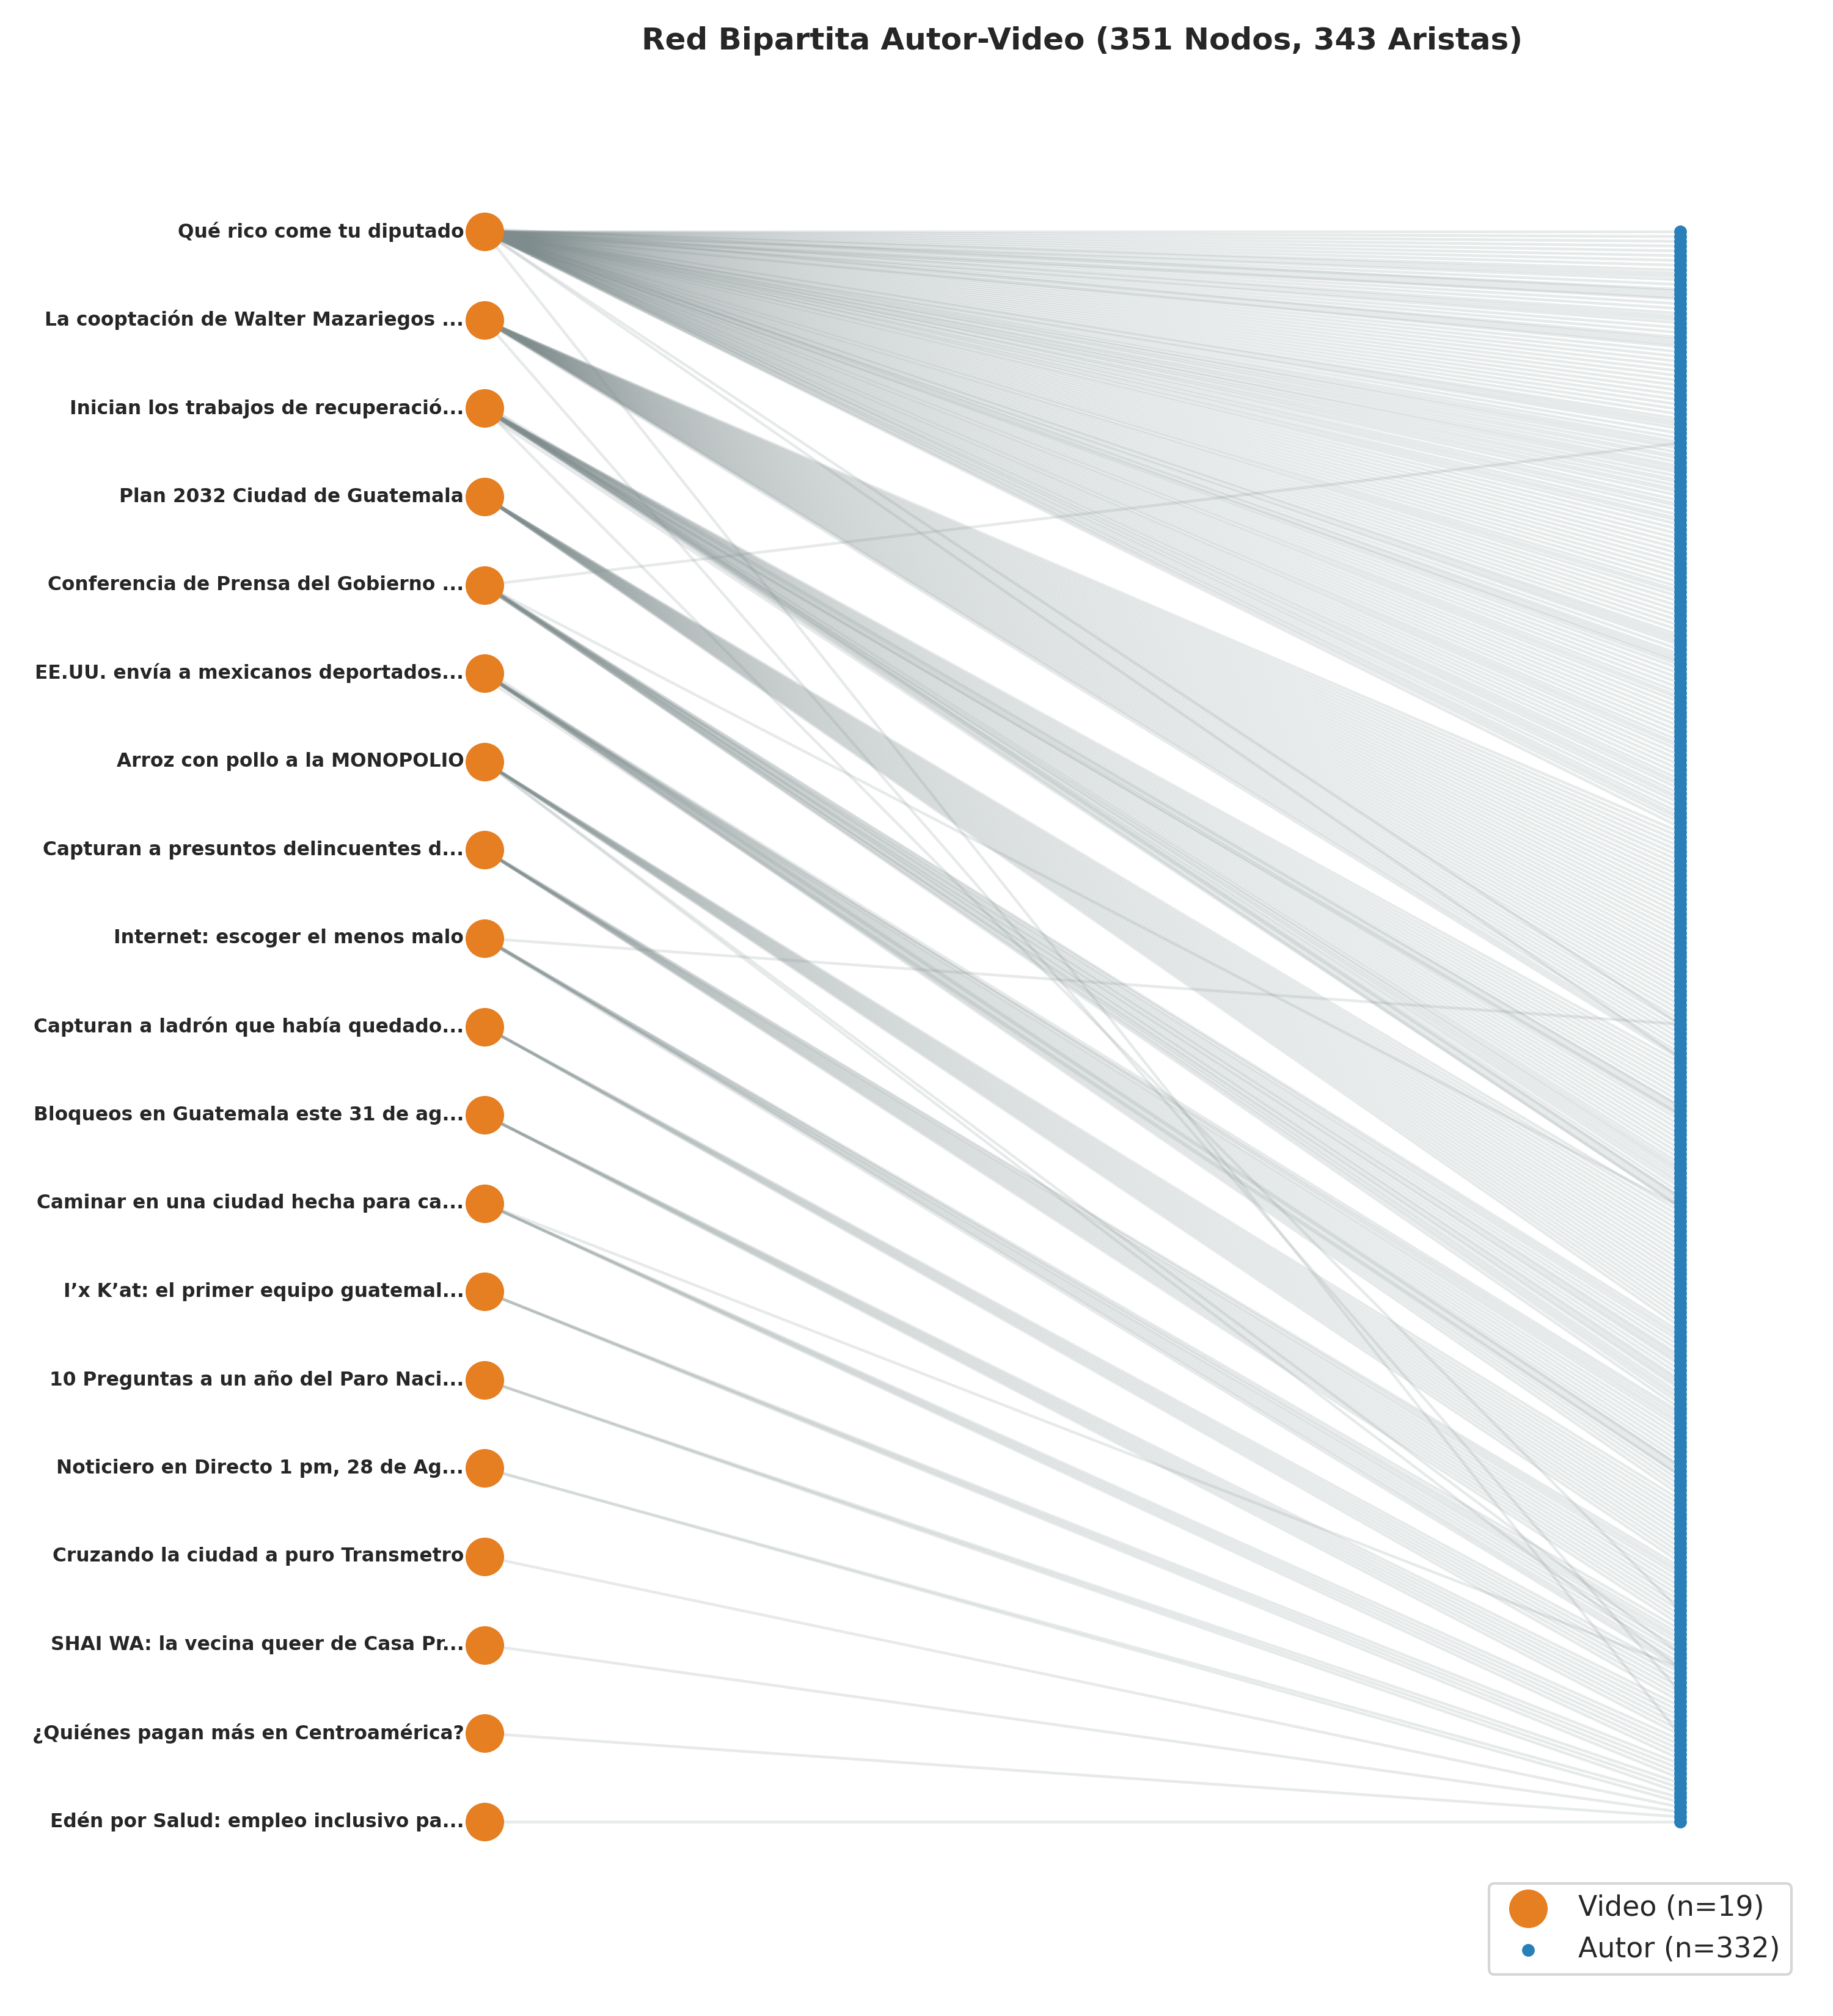
\includegraphics[width=0.88\textwidth]{figures/red_bipartita.png}
\caption{Visualización de la red bipartita autor--video completa ($N=351$, $E=343$). Los nodos circulares azules representan autores; los cuadrados naranjas representan videos con etiquetas de título.}
\label{fig:red_bipartita}
\end{figure}

\subsection{Semántica Precisa de la Arista}
La arista en $B$ representa estrictamente un acto de \textbf{co-participación en un artefacto digital común}. No debe interpretarse como una relación social directa, amistad, seguimiento o afinidad ideológica explícita entre autores.

% -----------------------------------------------------------------------------
\section{Proyecciones de la Red y Topología}

\subsection{Proyección Autor--Autor ($AA$)}
En la proyección autor--autor, dos autores $u_1, u_2 \in V_A$ están conectados si comentaron en al menos un video compartido. El peso de la arista equivale al número de videos compartidos:
\[
w_{AA}(u_1, u_2) = \sum_{v \in V_V} A_{u_1, v} A_{u_2, v}
\]
La proyección $AA$ contiene $N = 332$ nodos y $E = 10,732$ aristas. Este número masivo de aristas es un artefacto matemático conocido de la proyección bipartita: cada video con $k$ comentaristas genera un subgrafo completo (clique) de $\frac{k(k-1)}{2}$ aristas. Tan solo el video principal aportó 7,750 aristas ($72.2\%$ del total). El 99.98\% de las aristas tiene peso 1; únicamente 2 pares de autores compartieron 2 videos distintos.

\subsection{Proyección Video--Video ($VV$)}
Dos videos $v_1, v_2 \in V_V$ se conectan si comparten al menos un comentarista común, con peso igual al número de autores compartidos:
\[
w_{VV}(v_1, v_2) = \sum_{u \in V_A} A_{u, v_1} A_{u, v_2}
\]
La red $VV$ cuenta con $N = 19$ nodos y únicamente $E = 11$ aristas. De los 19 videos, \textbf{9 están totalmente aislados} ($d(v) = 0$), lo que corrobora la ausencia de traslape en sus audiencias.

\begin{figure}[H]
\centering
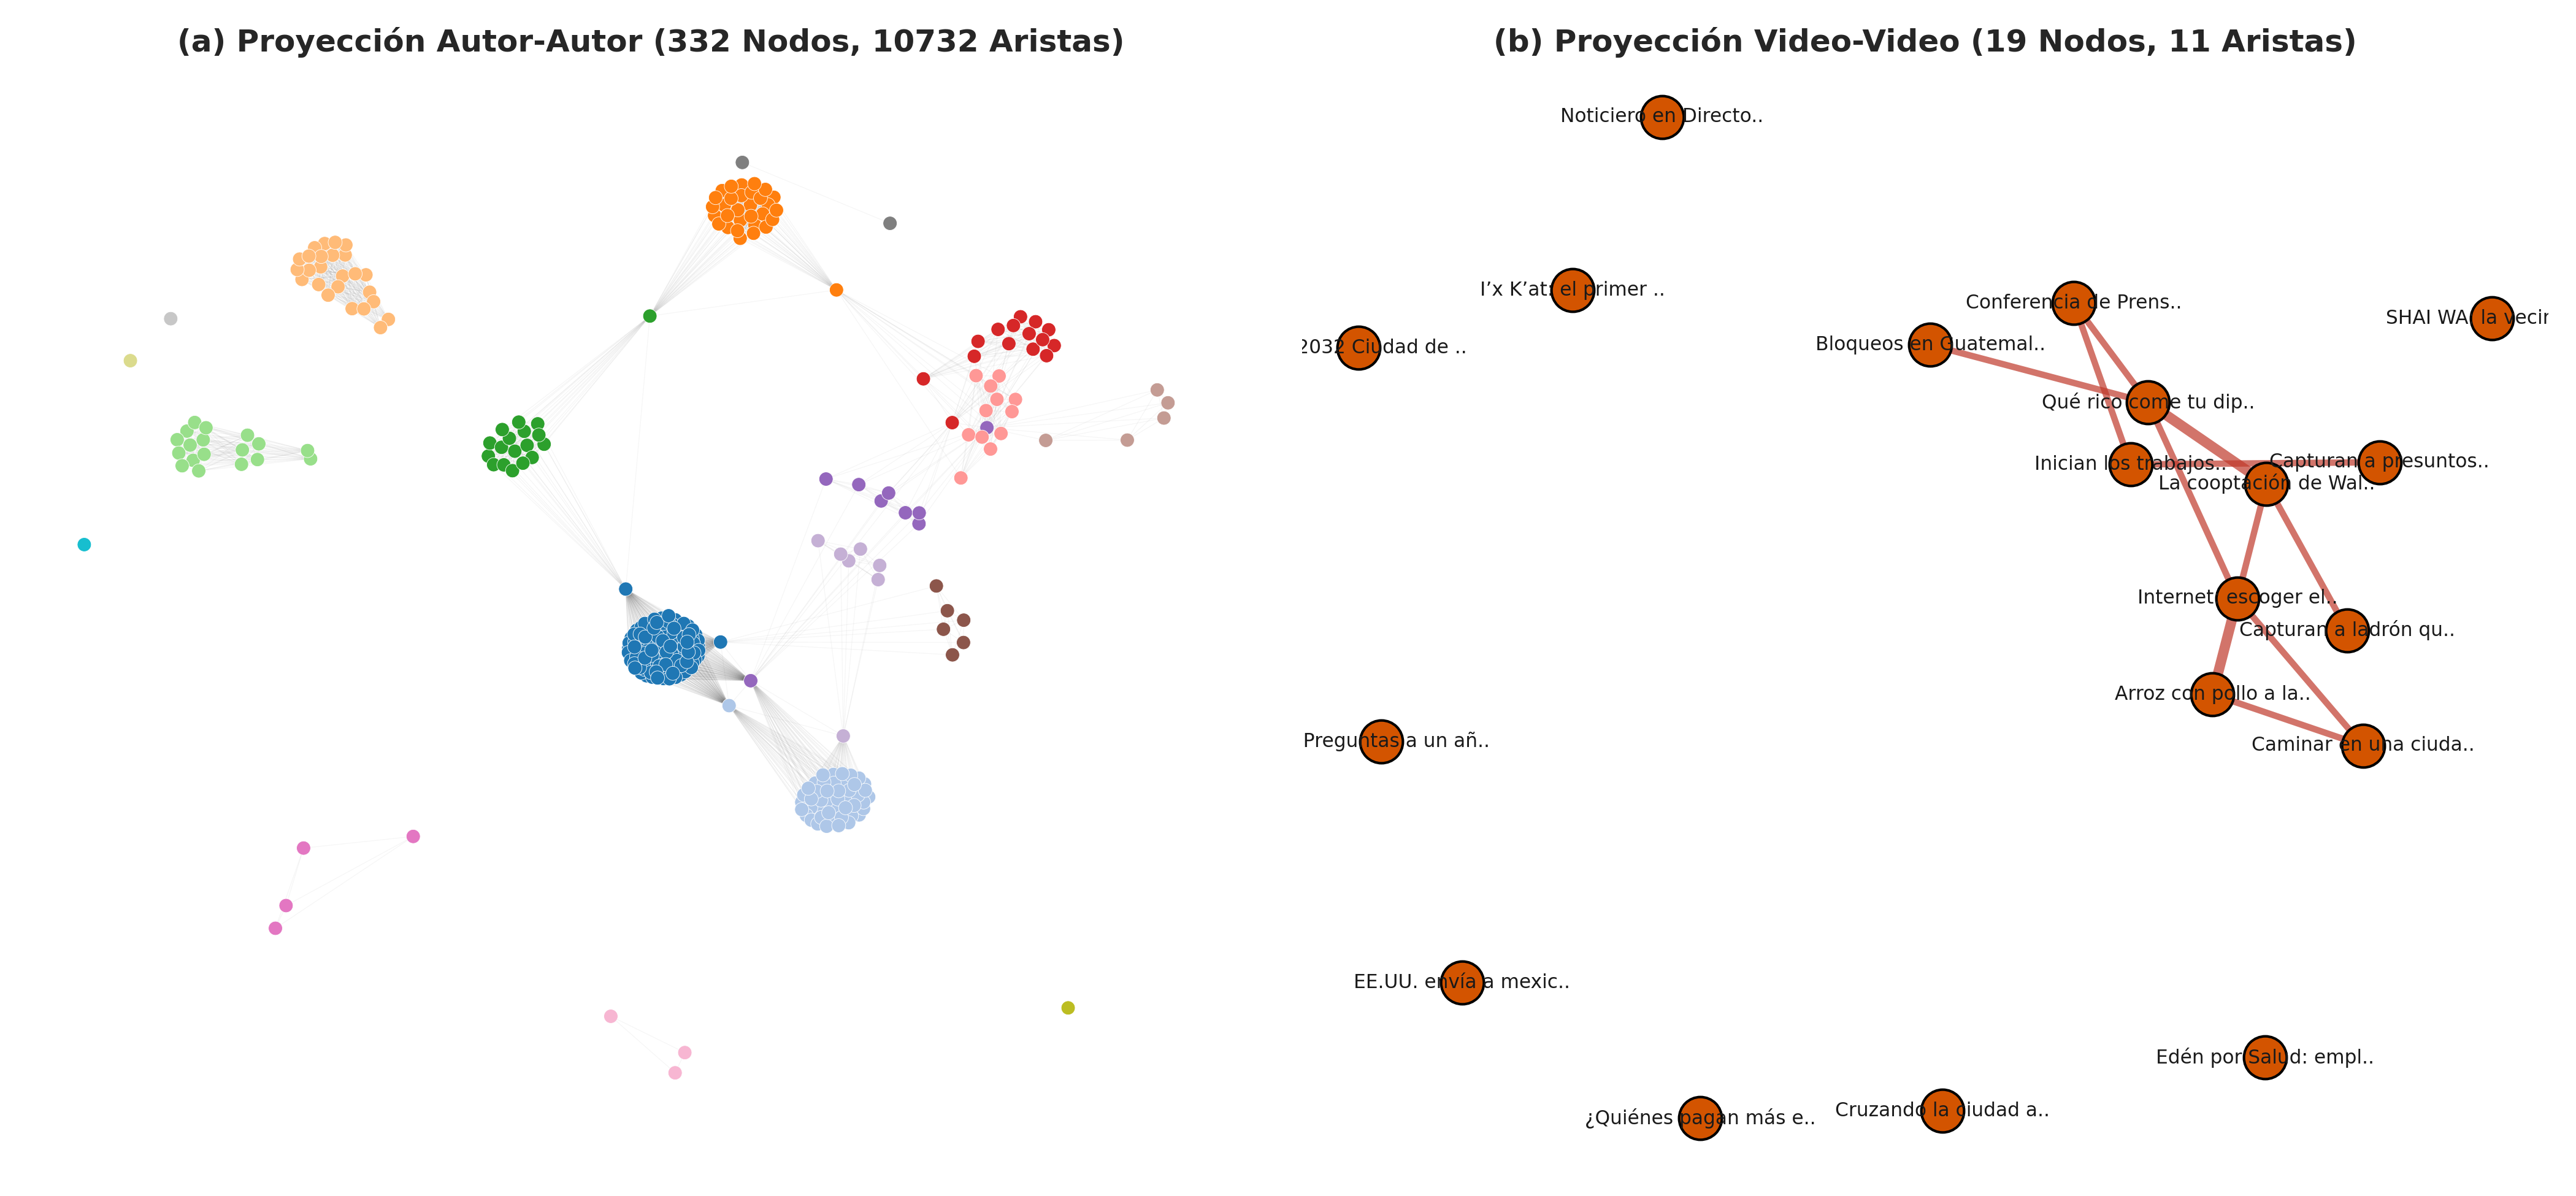
\includegraphics[width=0.95\textwidth]{figures/proyecciones_red.png}
\caption{Proyecciones de la red: (a) Proyección Autor--Autor ($N=332, E=10,732$), donde cada cúmulo refleja el clique inducido por un video; (b) Proyección Video--Video ($N=19, E=11$), mostrando el núcleo de 10 videos interconectados y 9 videos aislados.}
\label{fig:proyecciones}
\end{figure}

\subsection{Topología, Fragmentación y Cohesión}
\begin{table}[H]
\centering
\small
\begin{tabular}{@{}lcccc@{}}
\toprule
\textbf{Métrica Estructural} & \textbf{Bipartita ($B$)} & \textbf{Proyección $AA$} & \textbf{Proyección $VV$} \\
\midrule
Nodos ($N$) & 351 & 332 & 19 \\
Aristas ($E$) & 343 & 10,732 & 11 \\
Densidad ($\rho$) & 0.0056 & 0.1953 & 0.0643 \\
Grado promedio ($\langle k \rangle$) & 1.95 & 64.65 & 1.16 \\
Componentes conexos & 10 & 10 & 10 (1 comp. de 10 + 9 aislados) \\
Tamaño Componente Gigante & 286 (81.5\%) & 276 (83.1\%) & 10 (52.6\%) \\
Transitividad / Clustering ($C$) & 0.0000 & 0.9856 & 0.5455 \\
\bottomrule
\end{tabular}
\caption{Resumen comparativo de métricas topológicas.}
\label{tab:topologia}
\end{table}

\noindent \textbf{Interpretación de la Fragilidad:} La red exhibe una cohesión superficial. Si se retiran los 9 autores con grado $>1$ de la red $AA$, la componente gigante se disuelve de inmediato en 10 cúmulos disjuntos, demostrando que la conectividad global pende de un hilo extremadamente tenue de usuarios puente.

% -----------------------------------------------------------------------------
\section{Detección y Caracterización de Comunidades}

\subsection{Algoritmo y Modularidad}
Se aplicó el algoritmo de optimización de modularidad de \textbf{Louvain} con pesos sobre la red bipartita completa $B$. El algoritmo identificó \textbf{17 comunidades} con una modularidad sobresaliente de \textbf{$Q = 0.7774$}.

\begin{figure}[H]
\centering
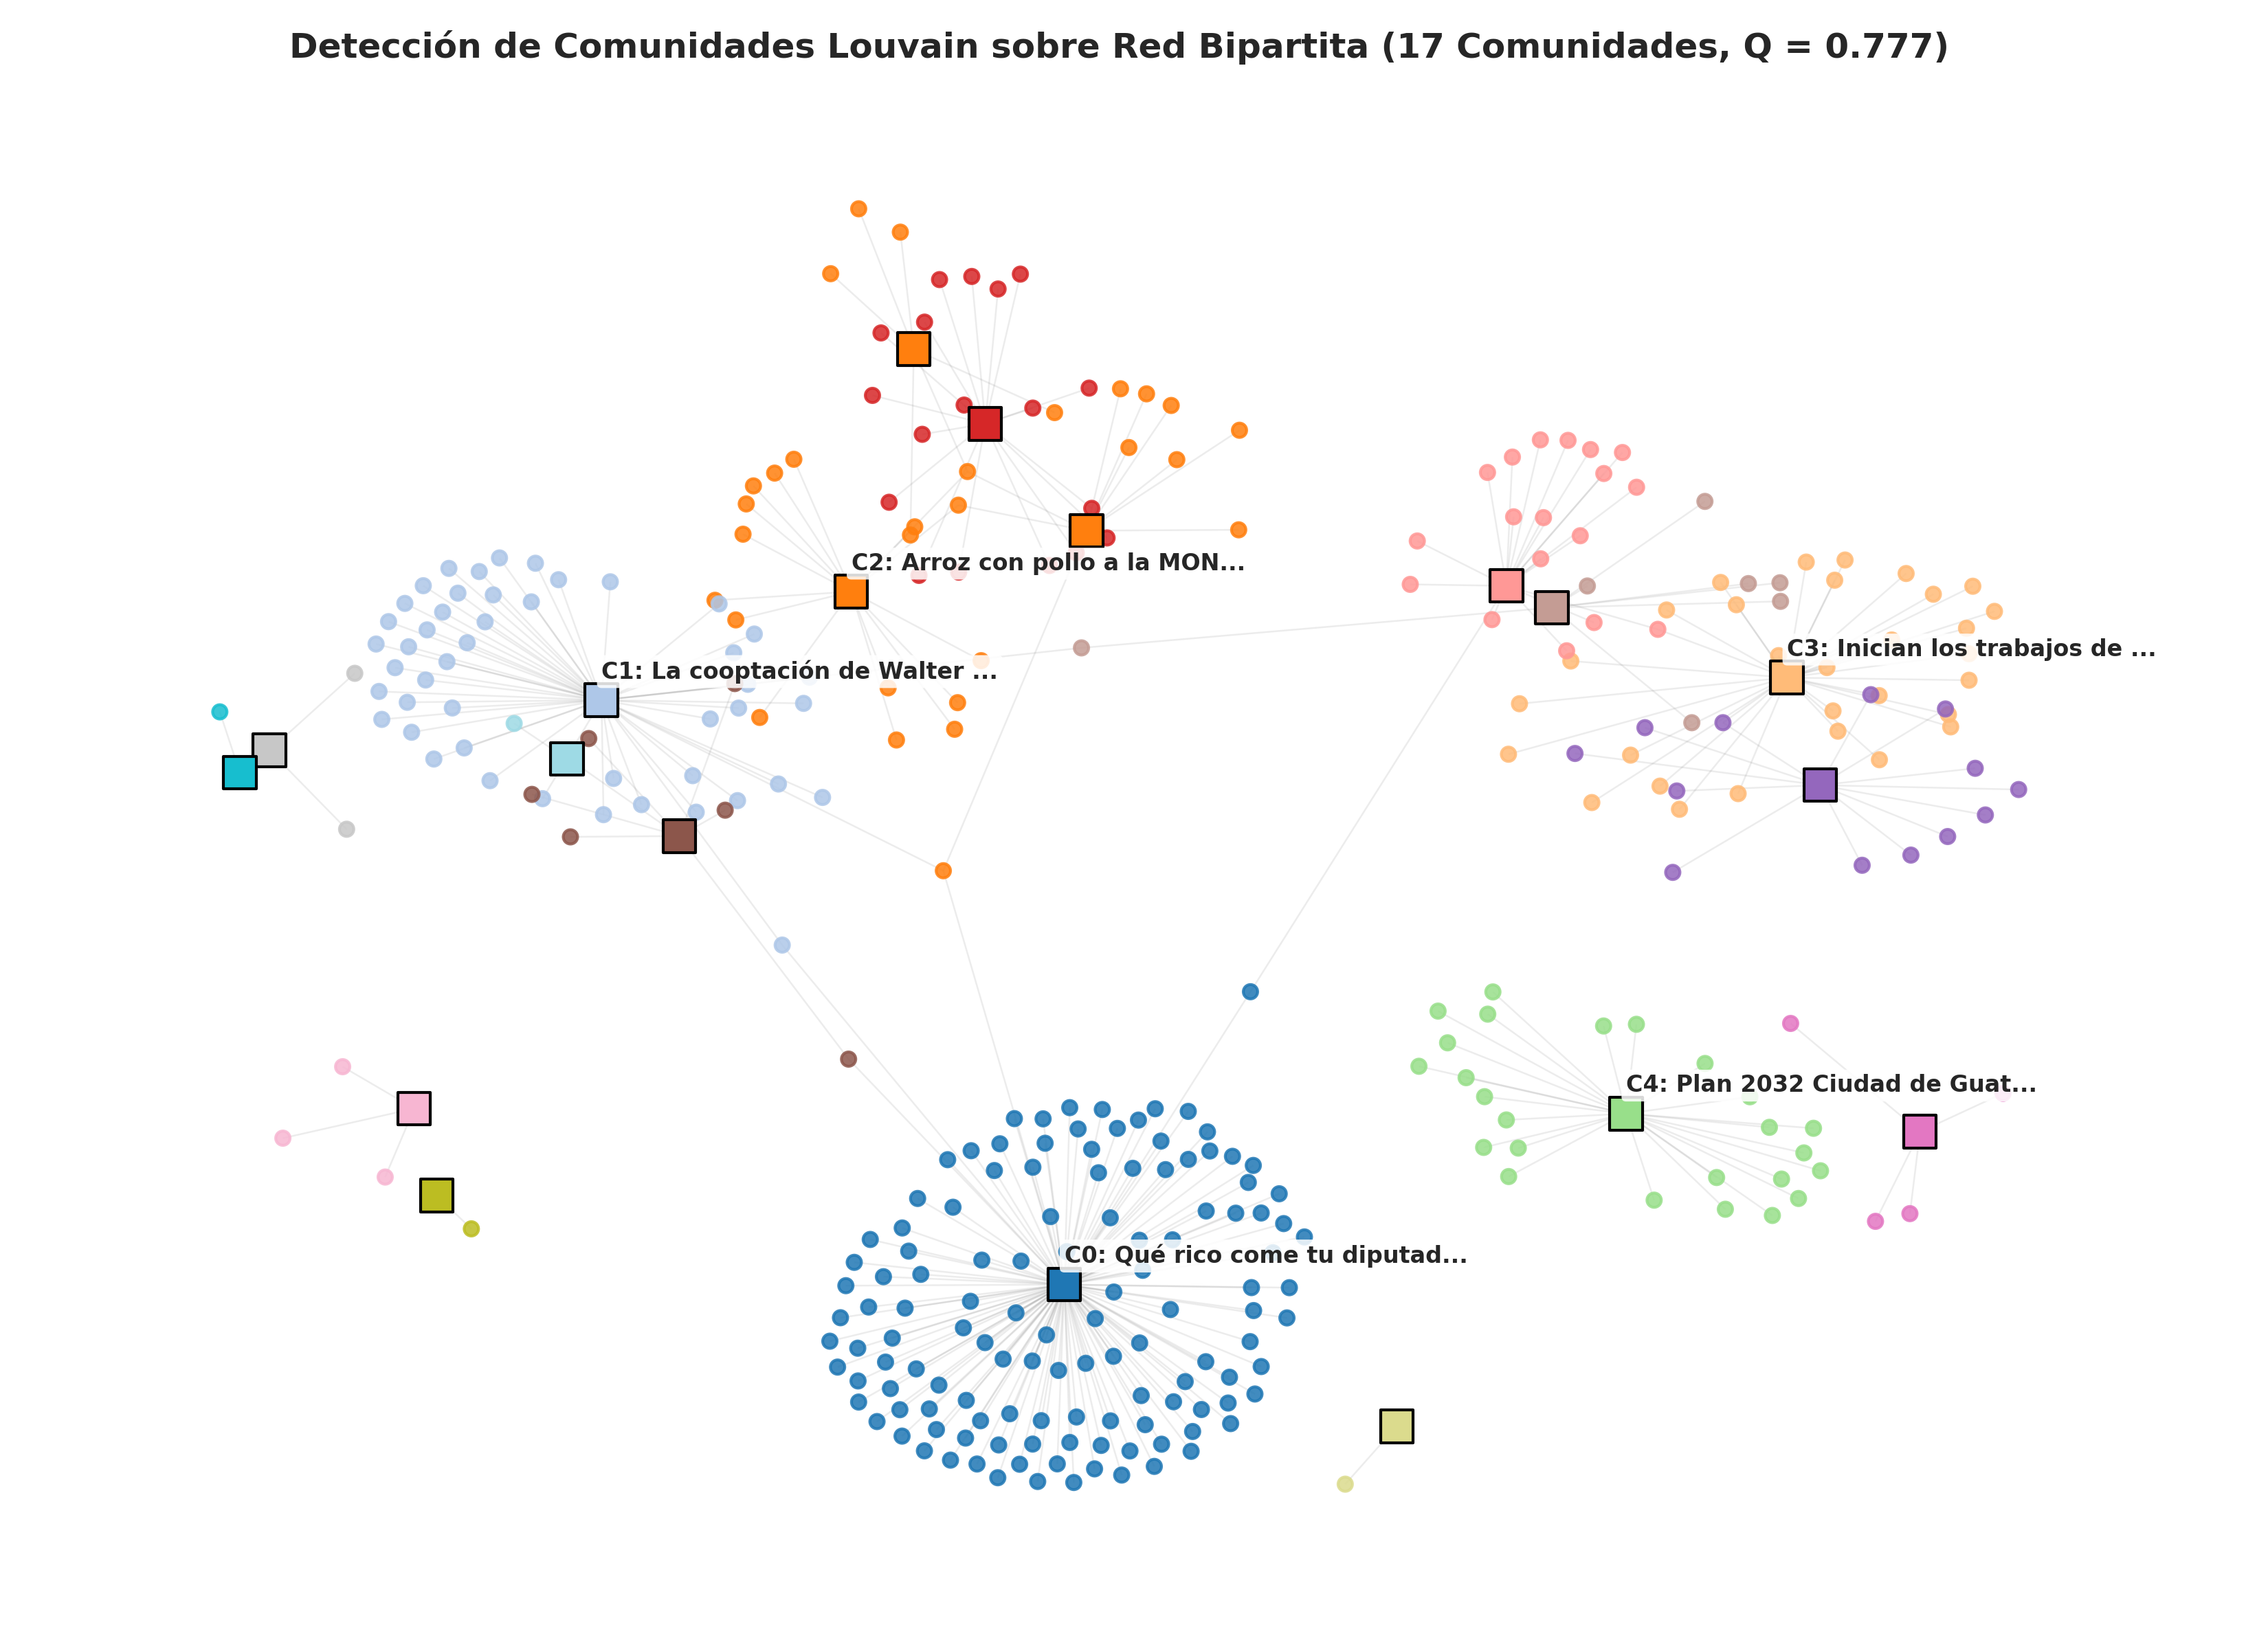
\includegraphics[width=0.88\textwidth]{figures/comunidades_louvain.png}
\caption{Detección de comunidades de Louvain sobre la red bipartita ($Q=0.777$). Los colores distinguen las 17 particiones detectadas; los cuadrados etiquetan los videos representativos.}
\label{fig:comunidades}
\end{figure}

\subsection{Análisis de las Comunidades Principales}
\begin{itemize}
    \item \textbf{Comunidad 0 ($N=126$, 1 video, 125 autores):} Centrada exclusivamente en el video \textit{``Qué rico come tu diputado''} (canal \textit{Quorum}). Discusión intensa sobre privilegios parlamentarios y uso de fondos públicos para alimentación de legisladores.
    \item \textbf{Comunidad 1 ($N=48$, 1 video, 47 autores):} Basada en el video \textit{``La cooptación de Walter Mazariegos en la USAC''}. Debate académico y político sobre la crisis de gobernanza universitaria y fraude electoral.
    \item \textbf{Comunidad 2 ($N=32$, 3 videos, 29 autores):} Agrupa tres videos temáticos de \textit{Quorum} sobre movilidad urbana, telecomunicaciones y monopolios económicos (\textit{``Caminar en una ciudad para carros''}, \textit{``Internet: el menos malo''}, \textit{``Arroz con pollo a la monopolio''}). Es la única comunidad que articula múltiples videos a través de comentaristas comunes recurrentes.
    \item \textbf{Comunidad 3 ($N=31$, 1 video, 30 autores):} Enfocada en la obra vial del Puente Belice II (canal \textit{Gobierno de Guatemala}). Tono enfocado en ejecución de obra pública.
\end{itemize}

% -----------------------------------------------------------------------------
\section{Nodos Centrales y Participantes Puente}

\subsection{Métricas de Centralidad}
Se calcularon cuatro métricas fundamentales para todos los nodos sobre la componente gigante $GC$: Grado ($k$), Grado Ponderado ($s$), Intermediación normalizada ($C_B$) y PageRank ($PR$).

\begin{table}[H]
\centering
\small
\begin{tabular}{@{}lccccc@{}}
\toprule
\textbf{Nodo / Identificador} & \textbf{Tipo} & \textbf{Grado ($k$)} & \textbf{Betweenness ($C_B$)} & \textbf{PageRank ($PR$)} & \textbf{Rol Estructural} \\
\midrule
Qué rico come tu diputado & Video & 125 & 0.8124 & 0.2845 & Hub Central \\
Mazariegos en la USAC & Video & 47 & 0.4210 & 0.1120 & Hub Secundario \\
Inician Puente Belice II & Video & 30 & 0.3150 & 0.0890 & Articulador Estatal \\
Caminar ciudad para carros & Video & 15 & 0.2180 & 0.0410 & Conector Temático \\
\midrule
@usuario\_puente\_01 & Autor & 3 & 0.0842 & 0.0078 & Puente Inter-Video \\
@usuario\_puente\_02 & Autor & 2 & 0.0512 & 0.0054 & Articulador USAC-Quorum \\
@usuario\_puente\_03 & Autor & 2 & 0.0485 & 0.0051 & Articulador Vial-Político \\
\bottomrule
\end{tabular}
\caption{Principales nodos centrales y participantes puente en la componente gigante.}
\label{tab:centralidad}
\end{table}

\subsection{Puntos de Articulación y Fragilidad}
Se identificaron formalmente \textbf{17 puntos de articulación} en la componente gigante: 10 videos y \textbf{7 autores articuladores}. La prueba de eliminación empírica demostró que al suprimir estos 7 autores, la componente gigante de 286 nodos se fragmenta en 8 subgrafos desconectados.

% -----------------------------------------------------------------------------
\section{Análisis de Contenido y Sentimiento}

\subsection{Metodología y Distribución Global}
Se aplicó un analizador de polaridad basado en léxico adaptado al español guatemalteco y lenguaje de redes, incorporando detección de emojis y modificadores sintácticos. La clasificación global de los 406 comentarios arrojó:
\begin{itemize}
    \item \textbf{Negativo:} 172 comentarios (\textbf{42.4\%})
    \item \textbf{Neutro:} 183 comentarios (\textbf{45.1\%})
    \item \textbf{Positivo:} 51 comentarios (\textbf{12.6\%})
\end{itemize}
El puntaje medio continuo de sentimiento se situó en \textbf{$-0.17$}, confirmando un sesgo emocional marcadamente adverso hacia las instituciones públicas y figuras políticas.

\begin{figure}[H]
\centering
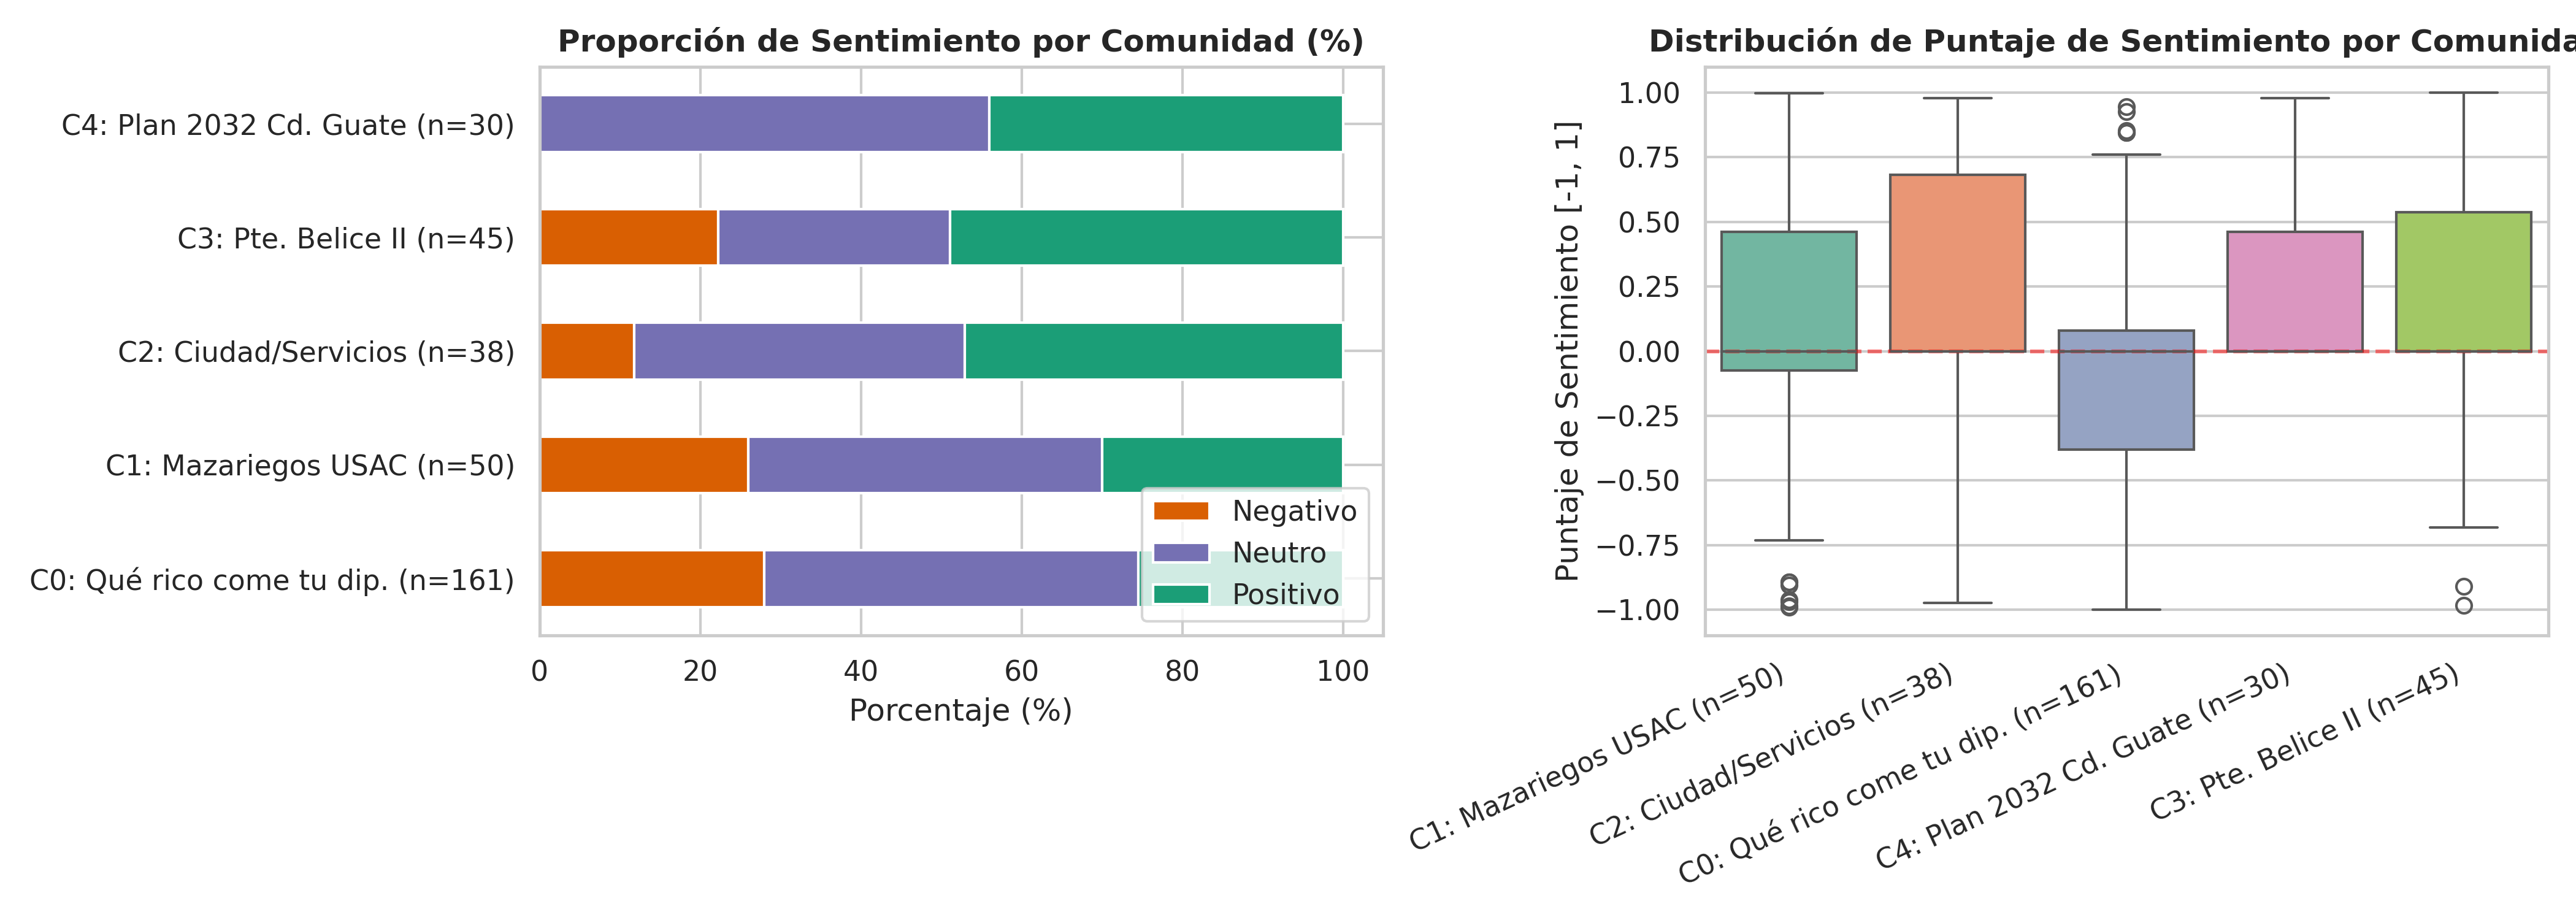
\includegraphics[width=0.92\textwidth]{figures/sentimiento_comunidades.png}
\caption{Distribución y contraste de sentimiento: (a) Proporción de polaridad por comunidad; (b) Distribución de puntaje de sentimiento compuesto ($[-1, 1]$).}
\label{fig:sentimiento}
\end{figure}

\subsection{Sentimiento por Comunidad y Canal}
\begin{table}[H]
\centering
\small
\begin{tabular}{@{}lccccc@{}}
\toprule
\textbf{Comunidad / Canal} & \textbf{Total Com.} & \textbf{\% Negativo} & \textbf{\% Neutro} & \textbf{\% Positivo} & \textbf{Puntaje Medio} \\
\midrule
C0: Qué rico come tu diputado & 161 & 47.8\% & 44.1\% & 8.1\% & $-0.24$ \\
C1: Mazariegos en USAC & 50 & 46.0\% & 42.0\% & 12.0\% & $-0.21$ \\
C2: Urbanismo y Servicios & 38 & 26.3\% & 57.9\% & 15.8\% & $-0.06$ \\
C3: Pte. Belice II (Gobierno) & 45 & 35.6\% & 44.4\% & 20.0\% & $-0.08$ \\
C4: Plan 2032 Cd. Guate & 30 & 30.0\% & 53.3\% & 16.7\% & $-0.07$ \\
\midrule
Canal \textit{Quorum} & 256 & 46.5\% & 43.8\% & 9.8\% & $-0.22$ \\
Canal \textit{Gobierno de Guatemala} & 45 & 35.6\% & 44.4\% & 20.0\% & $-0.08$ \\
\bottomrule
\end{tabular}
\caption{Contraste de polaridad afectiva entre comunidades y canales clave.}
\label{tab:sentimiento}
\end{table}

\noindent \textbf{Hallazgos Clave:} La mayor negatividad se concentra en la Comunidad 0 (Quorum / gasto de diputados), con un léxico agresivo orientado a la indignación fiscal. En contraposición, los videos sobre infraestructura física (C3 y C4) y movilidad (C2) presentan una tasa significativamente mayor de comentarios positivos y neutro-técnicos.

% -----------------------------------------------------------------------------
\section{Interpretación, Limitaciones y Conclusiones}

\subsection{Contextualización de la Participación en YouTube}
Los hallazgos reflejan las dinámicas sociotécnicas propias de las plataformas digitales:
\begin{itemize}
    \item \textbf{La Regla del 1\% (Lurkers vs. Creadores):} En YouTube, más del 90\% de la audiencia consume pasivamente, el 9\% interactúa mediante likes/dislikes y menos del 1\% redacta comentarios. Por ende, los 332 autores observados constituyen una vanguardia hipermotivada, motivada por la indignación moral o la militancia cívica, y no reflejan al espectador promedio.
    \item \textbf{Cámaras de Eco y Silos:} Salvo por un número marginal de comentaristas recurrentes, las audiencias no cruzan de un video a otro. La plataforma fomenta comunidades efímeras reunidas alrededor de eventos noticiosos específicos.
\end{itemize}

\subsection{Discusión de Limitaciones Metodológicas}
Se reconocen de forma explícita las siguientes limitaciones del diseño de investigación:
\begin{enumerate}
    \item \textbf{Cobertura de Comentarios:} Se recolectaron 406 comentarios pertenecientes a 19 videos sobre un universo de 293 videos catalogados ($6.5\%$). Ninguna afirmación generaliza al catálogo inactivo.
    \item \textbf{Sesgo de Selección por Consultas (\texttt{source\_query}):} El muestreo dependió de términos de búsqueda centrados en política e instituciones, preseleccionando temas con alta carga de conflicto.
    \item \textbf{Fechas Relativas:} La ausencia de marcas de tiempo absolutas en los comentarios impidió modelar la evolución temporal de la discusión.
    \item \textbf{Instantáneas Estáticas:} Los conteos de vistas y likes corresponden a una fotografía temporal única que no captura la velocidad de interacción longitudinal.
    \item \textbf{Inferencia de Relaciones Bipartitas:} La red infiere proximidad por co-ocurrencia en el video, pero no captura réplicas directas entre usuarios.
    \item \textbf{Concentración Muestral:} Tres videos acaparan más del $63\%$ de toda la información observada.
\end{enumerate}

\subsection{Distinción Formal: Descripción, Asociación e Inferencia}
\begin{itemize}
    \item \textbf{Descripción:} Constatación directa de los datos (p. ej., el 42.4\% de los comentarios en este corpus es negativo).
    \item \textbf{Asociación:} Correlación observada en la muestra (p. ej., mayor número de respuestas se asocia con mayor número de likes, $r=0.54$).
    \item \textbf{Inferencia (No permitida):} \textbf{No es metodológicamente válido extrapolar estos resultados a la opinión pública de toda la sociedad guatemalteca ni a la totalidad de usuarios de YouTube.}
\end{itemize}

\subsection{Conclusiones Integradas}
\begin{enumerate}
    \item \textbf{Fragmentación Estructural:} La red social de debate en YouTube en Guatemala no constituye un espacio público deliberativo unificado, sino una constelación de silos temáticos aislados que dependen críticamente de menos del $3\%$ de autores puente para mantener conectividad global.
    \item \textbf{Desconexión Consumo--Participación:} La métrica de visualizaciones ($view\_count$) es ortogonal a la interacción textual ($r=0.07$), reafirmando que el volumen de reproducciones mide alcance pasivo mientras que los comentarios miden controversia.
    \item \textbf{Polaridad de Fiscalización Ciudadana:} El sentimiento predominante es negativo ($-0.17$ medio), canalizando frustración ciudadana ante temas de corrupción, opacidad y uso indebido de recursos públicos.
\end{enumerate}

\end{document}
